\section{Week 10}

\subsection{Limits and Colimits of Modules}

Suppose we have a category $\cJ$ and functor $F:\cJ \to \text{Module}_R$ as in the following:
\begin{figure}[H]
    \centering
    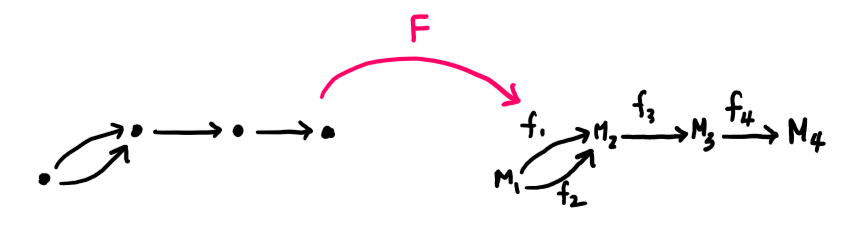
\includegraphics[width=0.6\linewidth]{figures/limit-1.png}
\end{figure}
($\cJ$ is usually thought as an index category.) The limit $A$ and colimit $B$ of $F$ are then defined as the $R$-modules
\begin{figure}[H]
    \centering
    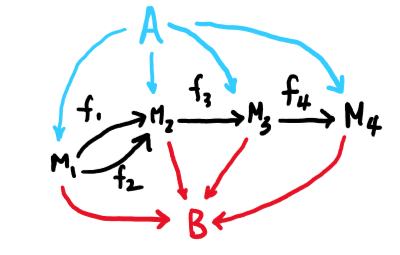
\includegraphics[width=0.3\linewidth]{figures/limit-2.png}
\end{figure}
such that:
\begin{enumerate}
    \item In the diagram, any composition of maps from $M_i$ to $A$ (or $B$) is the same. (However, note we cannot say the diagram is commutative, e.g. $f_1$ and $f_2$ can be different.) 
    \item If $A'$ satifies the previous property, then maps from $A'$ factor through $A$ via a unique map $A' \to A$. Similarly, if $B'$ satisfies the previous property, then maps to $B'$ factor through $B$ via a unique map $B \to B'$.
\end{enumerate}
\begin{figure}[H]
    \centering
    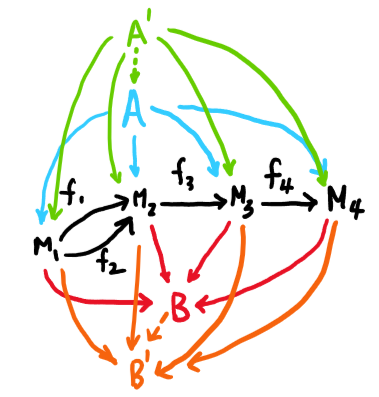
\includegraphics[width=0.3\linewidth]{figures/limit-3.png}
\end{figure}
Limits and colimits are general constructions found everywhere in math. With the correct choice of index category and functor, one can see that unions, direct sums, products, direct limits, and inverse limits are all examples of limits or colimits.

\subsection{Various Properties of Colimits}

For a given index category $\cJ$, we can view colimits as a functor on functors:
\[
    \colim_{\cJ}: (F: \cJ \to \text{Module}_R) \to \text{Module}_R.
\]
Call $\colim_{\cJ}$ exact if for all functors $A, B, C$ such that we have the mappings
\[
    0 \to A(i) \to B(i) \to C(i) \to 0, \quad \forall i \in \cJ,
\]
then the induced mappings on the colimits are exact:
\[
    0 \to \colim_{\cJ}A \to \colim_{\cJ}B \to \colim_{\cJ}C \to 0.
\]

\paragraph{Commutativity.} Colimits commmute in a Fubini-esque fashion, expressed by the following diagram:
\begin{figure}[H]
    \centering
    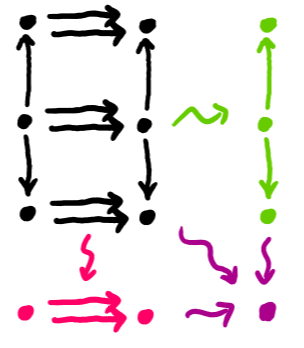
\includegraphics[width=0.2\linewidth]{figures/colim-comm.png}
\end{figure}
This is easy to verify and accounts for the commutativity of many different constructions arising from colimits. In particular, we can conclude that the quotient of colimits is the colimit of quotients, which proves the right-exactness of the colimit functor.

\paragraph{Filtered Colimits.} Call an category $\cJ$ filtered if:
\begin{enumerate}
    \item For $a, b \in \cJ$, there exists $c \in \cJ$ with maps $a \to c$, $b \to c$.
    \item For $a, b \in \cJ$, if there exists maps $f: a \to b$, $g: a \to b$, then there exists $c \in \cJ$ and $h: b \to c$ such that $hf = hg$.
\end{enumerate}
Note filtered categories are generalizations of directed posets. We call a colimit filtered if it uses a filtered index category.

One can show that a filtered colimit of modules $M_i$ is equal to
\[
    \frac{\bigsqcup M_i}{m_i \sim m_j \text{ if $m_i$ and $m_j$ map to same elem in some $M_k$}}.
\]
From this, one can conclude that filtered colimits preserve injectivity, so they are left-exact, and hence exact.

By commuting tensors with colimits, one can also see that filtered colimits of flat modules are flat.

\subsection{Limits and Exactness}
The proof that limits are left-exact is similar to the proof that colimits are right-exact. However, the full exactness of limits is harder to characterize. The analog of filtered colimits doesn't work; instead, we have the Mittag-Leffler condition, which we define (for simplicity) on the index category $\cJ =$
\[
    \bullet \leftarrow \bullet \leftarrow \bullet \leftarrow \bullet \leftarrow \dots
\]
as follows: we say functor $A$ on $\cJ$ has the M-L condition if the image of $A_j$ in $A_i$ stabilizes for large $j$, i.e. the chain
\[
    A_i \supset \Ima(A_{i+1}) \supset \Ima(A_{i+2}) \supset \dots
\]
eventually stabilizes.

It is a theorem that if $A,B,C$ are functors on $\cJ$ and $A$ satisfies the M-L condition, then the mappings
\[
    0 \to A(i) \to B(i) \to C(i) \to 0, \quad \forall i \in \cJ
\]
induce the exact sequence
\[
    0 \to \varprojlim_{\cJ}A \to \varprojlim_{\cJ}B \to \varprojlim_{\cJ}C \to 0.
\]
The proof can be broken into three steps:
\begin{enumerate}
    \item Via diagram chasing, we prove the case when $A_{i+1} \to A_i$ is always onto.
    \item Via diagram chasing, we prove the case when $A_{i+1} \to A_i$ eventually becomes trivial.
    \item Define $A_i' \subset A_i$ to be the stable limit of $A_{i+j}$ as $j \to \i$. One can show $A'_{i+1} \to A'_i$ is always onto, so by the first step, we have the right-derived functor
    \[
        \text{lim}^1(A_i') = 0.
    \]
    Similarly, analyzing $A_i/A_i'$ and applying the second step, we get
    \[
        \text{lim}^1(A_i/A_i') = 0.
    \]
    Then as the exact sequence $0 \to A'_i \to A_i \to A_i/A_i'$ gives rise to
    \[
        \text{lim}^1(A_i') \to \text{lim}^1(A_i) \to \text{lim}^1(A_i/A_i'),
    \]
    we conclude that $\text{lim}^1(A_i) = 0$, as claimed.
\end{enumerate}

\subsection{Completions Revisited}
Recall that the completion $\hat{R}$ of a ring $R$ w/r/t an ideal $I \subset R$ is defined as the limit of the rings
\[
    \frac{R}{I} \leftarrow \frac{R}{I^2} \leftarrow \frac{R}{I^3} \leftarrow \dots.
\]
Ring completion can also be reformulated in terms of metric space completion. We first turn $R$ into a metric space by defining the norm $|x| = C^{-n}$ for $x \in I^n$ but $x \not \in I^{n+1}$. Then one can show $\hat{R}$ is the metric space completion of $R$.

Because of this connection to metric space completion, one can expect $\hat{R}$ to behave like $\bR$. Indeed, we can often do analysis on $\hat{R}$ (e.g. define powers, gamma functions, etc.). Other advantages of working with completions are:
\begin{itemize}
    \item It is easy to solve equations in $\hat{R}$ (Hensel's Lemma).
    \item Completions are sort of a stronger form of localization (see below).
\end{itemize}

\paragraph{$p$-adic Integers.} The $p$-adic integers $\bZ_p$ are the completion of $\bZ$ w/r/t to prime ideal $(p)$. (We work with prime ideals because all $n$-adic numbers can be decomposed into the product of $p$-adic numbers for primes $p$.) For example, the $2$-adic integers consist of bit strings extending infinitely to the left.

Via the metric space interpretation, we note that two elements in the $p$-adic integers are close if their difference is divisble by a high power of $p$. This allows the $p$-adic numbers to encode information in a way that turns out to be very powerful in number theory.

\paragraph{Maximal Ideals.} Let $\hat{R}$ be the completion of $R$ w/r/t a maximal ideal $\mathfrak m$. One can show that elements in $R$ but not in $\mathfrak m$ are invertible in $\hat{R}$. Consequently, there is a natural map
\[
    R[\mathfrak m^{-1}] \to \hat{R}.
\]
In fact, one can view localization and completion as the first two steps of turning $R$ into a field:
\[
    R \to R[\mathfrak m^{-1}] \to \hat{R} \to \dots \to \frac{R}{\mathfrak m^2} \to \frac{R}{\mathfrak m}.
\]

%%% Local Variables:
%%% TeX-master: "main"
%%% End: